
\subsubsection{\textbf{Paralelización de los tres bucles:}}

%%% TABLA DE TIEMPOS E IMÁGENES %%%
\begin{figure}[H]
    \centering
    \begin{subfigure}{0.4\textwidth}
        \begin{adjustbox}{width=\textwidth} 
        \begin{tabular}{|c|c|c|c|c|}
            \hline
            \rowcolor{azul} \multicolumn{2}{|c|}{}&\multicolumn{3}{c|}{\textbf{Compiler}} \\ \hline
            \rowcolor{azul} \multicolumn{2}{|c|}{}&\texttt{clang}&\texttt{gcc}&\texttt{icc}\\ \hline
            \rowcolor{azul} \textbf{Testing size} & \textbf{Threads}&\multicolumn{3}{c|}{\textbf{Average time (s)}} \\ \hline
            \multirow{8}{1cm}{\textbf{01-small}} & 1 & \(1.53\pm{0.00}\) & \(0.38\pm{0.01}\) & \(1.01\pm{0.0}\) \\ \cline{2-5}
            & 2 & \(1.56\pm{0.00}\) & \(0.35\pm{0.01}\) & \(1.03\pm{0.01}\) \\ \cline{2-5}
            & 3 & \(1.58\pm{0.00}\) & \(0.34\pm{0.02}\) & \(1.06\pm{0.05}\) \\ \cline{2-5}
            & 4 & \(1.60\pm{0.00}\) & \(0.34\pm{0.02}\) & \(1.08\pm{0.01}\) \\ \cline{2-5}
            & 5 & \(1.73\pm{0.12}\) & \(0.47\pm{0.01}\) & \(1.42\pm{0.35}\) \\ \cline{2-5}
            & 6 & \(1.70\pm{0.10}\) & \(0.48\pm{0.01}\) & \(1.42\pm{0.35}\) \\ \cline{2-5}
            & 7 & \(1.73\pm{0.08}\) & \(0.48\pm{0.01}\) & \(1.46\pm{0.41}\) \\ \cline{2-5}
            & 8 & \(1.83\pm{0.02}\) & \(0.47\pm{0.01}\) & \(1.79\pm{0.02}\) \\ \hline
        \end{tabular}
        \end{adjustbox}
    \end{subfigure}
    \hfill
    \begin{subfigure}{0.5\textwidth}
        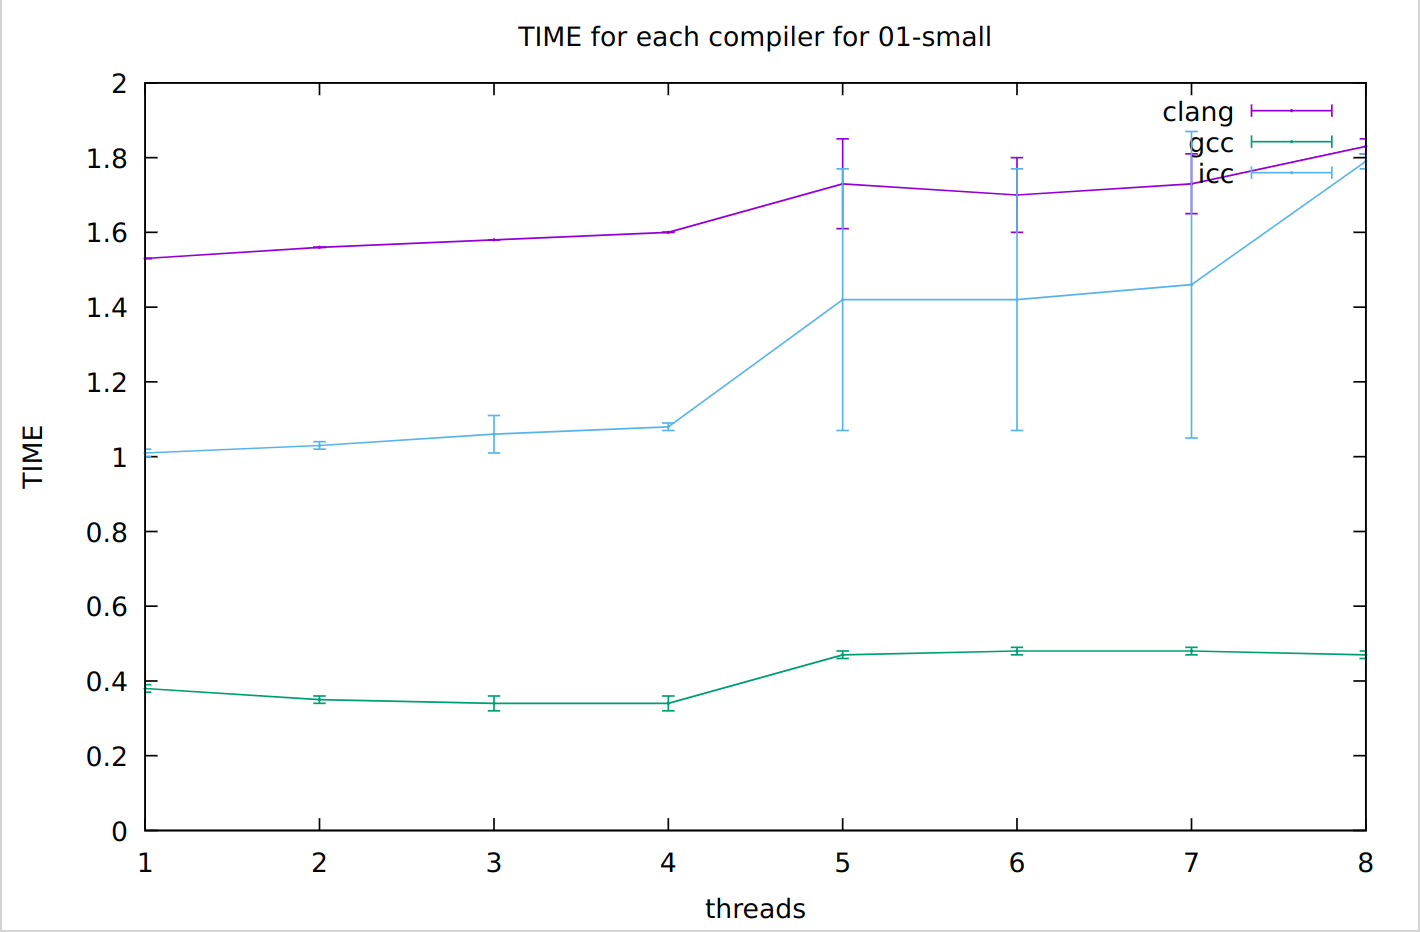
\includegraphics[width=\textwidth]{bucle1-2=01-small}
    \end{subfigure}
    \caption{\underline{Tamaño pequeño}: Tiempos de ejecución vs nº de hilos}
    \label{fig:bucle1-2=01-small}
\end{figure}

%%% TABLA DE TIEMPOS E IMÁGENES %%%
\begin{figure}[H]
    \centering
    \begin{subfigure}{0.4\textwidth}
        \begin{adjustbox}{width=\textwidth} 
        \begin{tabular}{|c|c|c|c|c|}
            \hline
            \rowcolor{azul} \multicolumn{2}{|c|}{}&\multicolumn{3}{c|}{\textbf{Compiler}} \\ \hline
            \rowcolor{azul} \multicolumn{2}{|c|}{}&\texttt{clang}&\texttt{gcc}&\texttt{icc}\\ \hline
            \rowcolor{azul} \textbf{Testing size} & \textbf{Threads}&\multicolumn{3}{c|}{\textbf{Average time (s)}} \\ \hline
            \multirow{8}{2.5cm}{\textbf{02-medium}} & 1 & \(4.50\pm{0.09}\) & \(0.88\pm{0.04}\) & \(2.94\pm{0.08}\) \\ \cline{2-5}
            & 2 & \(4.54\pm{0.03}\) & \(0.91\pm{0.04}\) & \(2.96\pm{0.04}\) \\ \cline{2-5}
            & 3 & \(4.53\pm{0.01}\) & \(0.91\pm{0.04}\) & \(2.97\pm{0.05}\) \\ \cline{2-5}
            & 4 & \(4.64\pm{0.02}\) & \(0.93\pm{0.04}\) & \(3.02\pm{0.04}\) \\ \cline{2-5}
            & 5 & \(4.68\pm{0.05}\) & \(0.94\pm{0.04}\) & \(3.03\pm{0.04}\) \\ \cline{2-5}
            & 6 & \(5.20\pm{0.02}\) & \(1.31\pm{0.03}\) & \(3.03\pm{0.04}\) \\ \cline{2-5}
            & 7 & \(5.25\pm{0.04}\) & \(1.30\pm{0.02}\) & \(5.15\pm{0.05}\) \\ \cline{2-5}
            & 8 & \(5.21\pm{0.00}\) & \(1.31\pm{0.03}\) & \(5.13\pm{0.06}\) \\ \hline
        \end{tabular}
        \end{adjustbox}
    \end{subfigure}
    \hfill
    \begin{subfigure}{0.5\textwidth}
        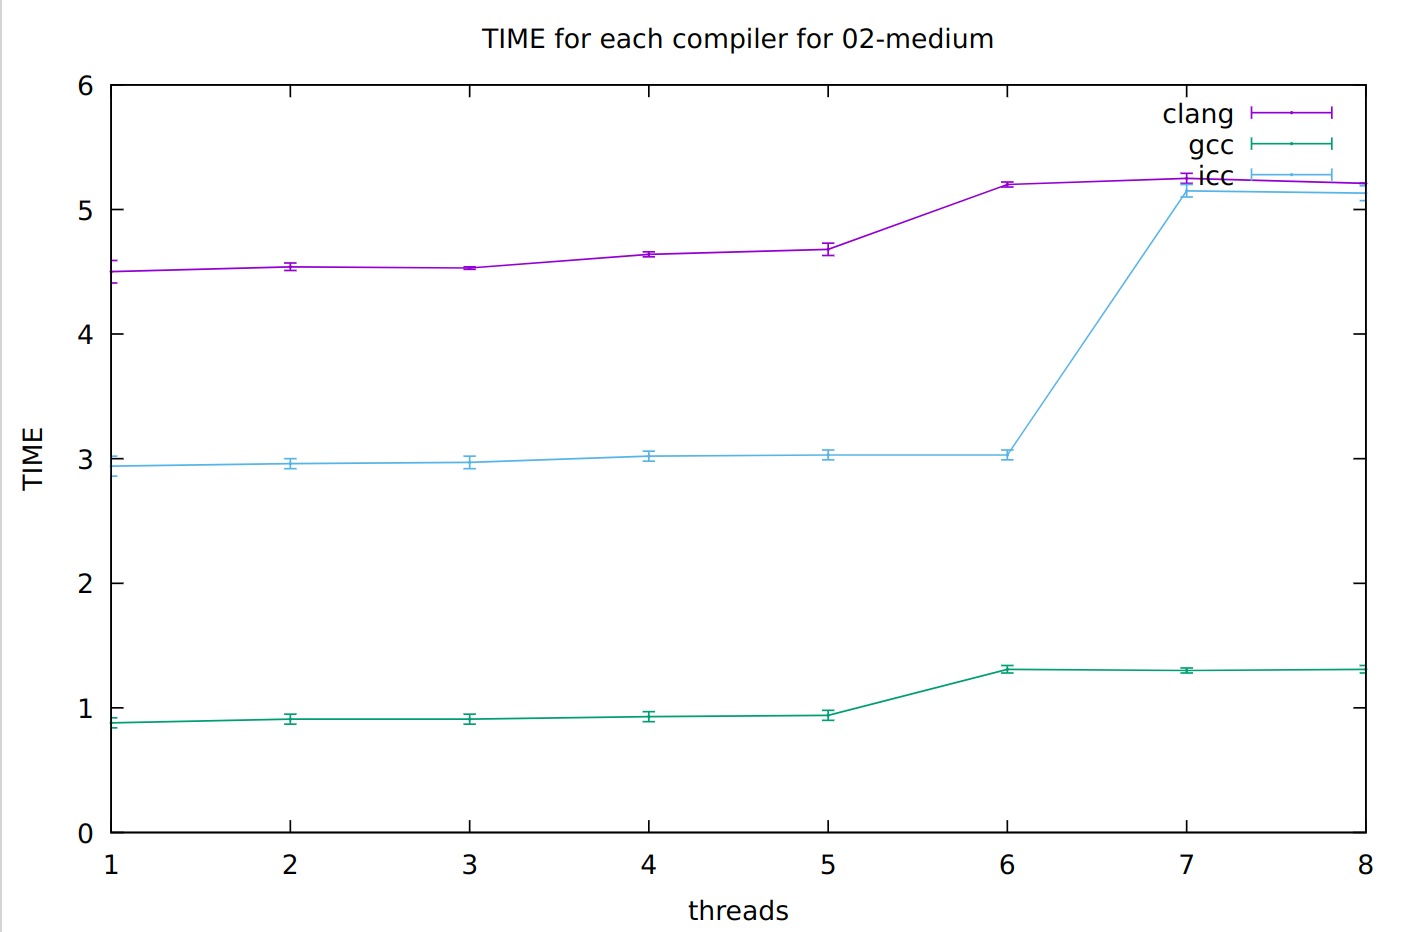
\includegraphics[width=\textwidth]{bucle1-2=02-medium}
    \end{subfigure}
    \caption{\underline{Tamaño mediano}: Tiempos de ejecución vs nº de hilos}
    \label{bucle1-2=02-medium}
\end{figure}

%%% TABLA DE TIEMPOS E IMÁGENES %%%
\begin{figure}[H]
    \centering
    \begin{subfigure}{0.4\textwidth}
        \begin{adjustbox}{width=\textwidth} 
        \begin{tabular}{|c|c|c|c|c|}
            \hline
            \rowcolor{azul} \multicolumn{2}{|c|}{}&\multicolumn{3}{c|}{\textbf{Compiler}} \\ \hline
            \rowcolor{azul} \multicolumn{2}{|c|}{}&\texttt{clang}&\texttt{gcc}&\texttt{icc}\\ \hline
            \rowcolor{azul} \textbf{Testing size} & \textbf{Threads}&\multicolumn{3}{c|}{\textbf{Average time (s)}} \\ \hline
            \multirow{8}{1cm}{\textbf{03-large}} & 1 & \(7.56\pm{0.02}\) & \(1.53\pm{0.08}\) & \(5.00\pm{0.11}\) \\ \cline{2-5}
            & 2 & \(7.78\pm{0.01}\) & \(1.57\pm{0.08}\) & \(5.07\pm{0.10}\) \\ \cline{2-5}
            & 3 & \(7.80\pm{0.04}\) & \(1.57\pm{0.08}\) & \(5.18\pm{0.21}\) \\ \cline{2-5}
            & 4 & \(7.92\pm{0.06}\) & \(1.61\pm{0.07}\) & \(5.22\pm{0.12}\) \\ \cline{2-5}
            & 5 & \(7.85\pm{0.02}\) & \(2.20\pm{0.04}\) & \(5.31\pm{0.19}\) \\ \cline{2-5}
            & 6 & \(8.89\pm{0.06}\) & \(1.62\pm{0.07}\) & \(5.16\pm{0.09}\) \\ \cline{2-5}
            & 7 & \(8.90\pm{0.02}\) & \(2.21\pm{0.04}\) & \(8.71\pm{0.04}\) \\ \cline{2-5}
            & 8 & \(8.83\pm{0.03}\) & \(2.21\pm{0.04}\) & \(8.75\pm{0.14}\) \\ \hline
        \end{tabular}
        \end{adjustbox}
    \end{subfigure}
    \hfill
    \begin{subfigure}{0.5\textwidth}
        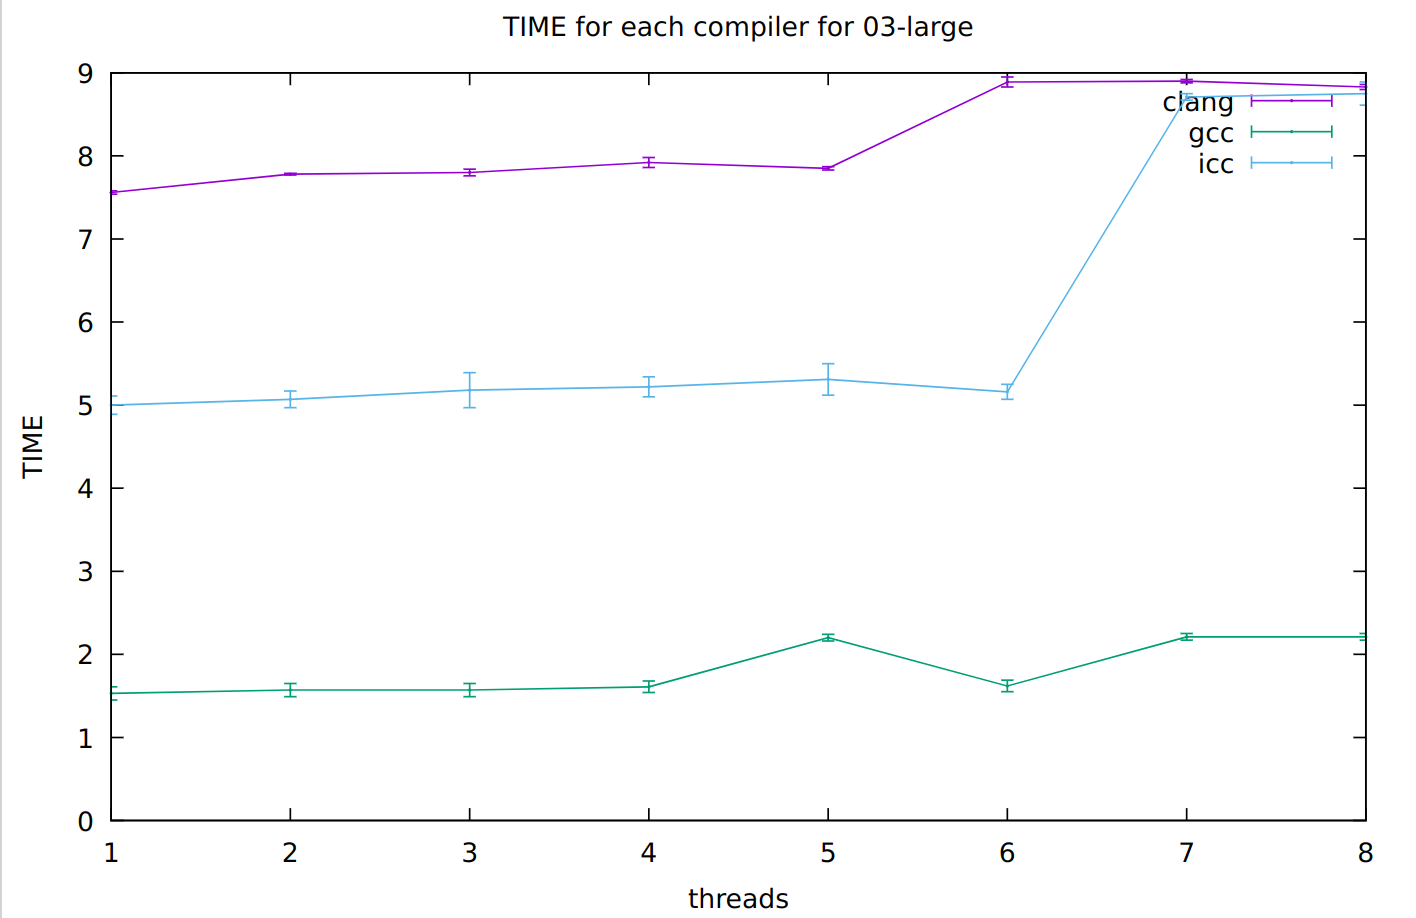
\includegraphics[width=\textwidth]{bucle1-2=03-large}
    \end{subfigure}
    \caption{\underline{Tamaño largo}: Tiempos de ejecución vs nº de hilos}
    \label{bucle1-2=03-large}
\end{figure}

%%%%%%%%%%%%%%%%%%%%%%%%%%%%%%%%%%%%%%%%%%%%%%%%%%%%%%%%%%%%%%%%%%%%%%%%%%%%%%%%%
%%% TABLA DE TIEMPOS E IMÁGENES %%%
\begin{figure}[H]
    \centering
    \begin{subfigure}{0.4\textwidth}
        \begin{adjustbox}{width=\textwidth} 
        \begin{tabular}{|c|c|c|c|c|}
            \hline
            \rowcolor{azul} \multicolumn{2}{|c|}{}&\multicolumn{3}{c|}{\textbf{Compiler}} \\ \hline
            \rowcolor{azul} \multicolumn{2}{|c|}{}&\texttt{clang}&\texttt{gcc}&\texttt{icc}\\ \hline
            \rowcolor{azul} \textbf{Testing size} & \textbf{Threads}&\multicolumn{3}{c|}{\textbf{Average time (s)}} \\ \hline
            \multirow{8}{1cm}{\textbf{01-small}} & 1 & \(3.36\pm{0.02}\) & \(1.80\pm{0.38}\) & \(5.68\pm{0.01}\) \\ \cline{2-5}
            & 2 & \(1.74\pm{0.01}\) & \(0.72\pm{0.01}\) & \(2.93\pm{0.01}\) \\ \cline{2-5}
            & 3 & \(1.19\pm{0.02}\) & \(0.50\pm{0.01}\) & \(1.98\pm{0.01}\) \\ \cline{2-5}
            & 4 & \(0.91\pm{0.01}\) & \(0.39\pm{0.01}\) & \(1.52\pm{0.01}\) \\ \cline{2-5}
            & 5 & \(1.35\pm{0.00}\) & \(0.59\pm{0.00}\) & \(2.21\pm{0.00}\) \\ \cline{2-5}
            & 6 & \(1.13\pm{0.00}\) & \(0.49\pm{0.00}\) & \(1.85\pm{0.01}\) \\ \cline{2-5}
            & 7 & \(0.98\pm{0.01}\) & \(0.43\pm{0.00}\) & \(1.60\pm{0.01}\) \\ \cline{2-5}
            & 8 & \(0.87\pm{0.00}\) & \(0.40\pm{0.01}\) & \(1.44\pm{0.03}\) \\ \hline
        \end{tabular}
        \end{adjustbox}
    \end{subfigure}
    \hfill
    \begin{subfigure}{0.5\textwidth}
        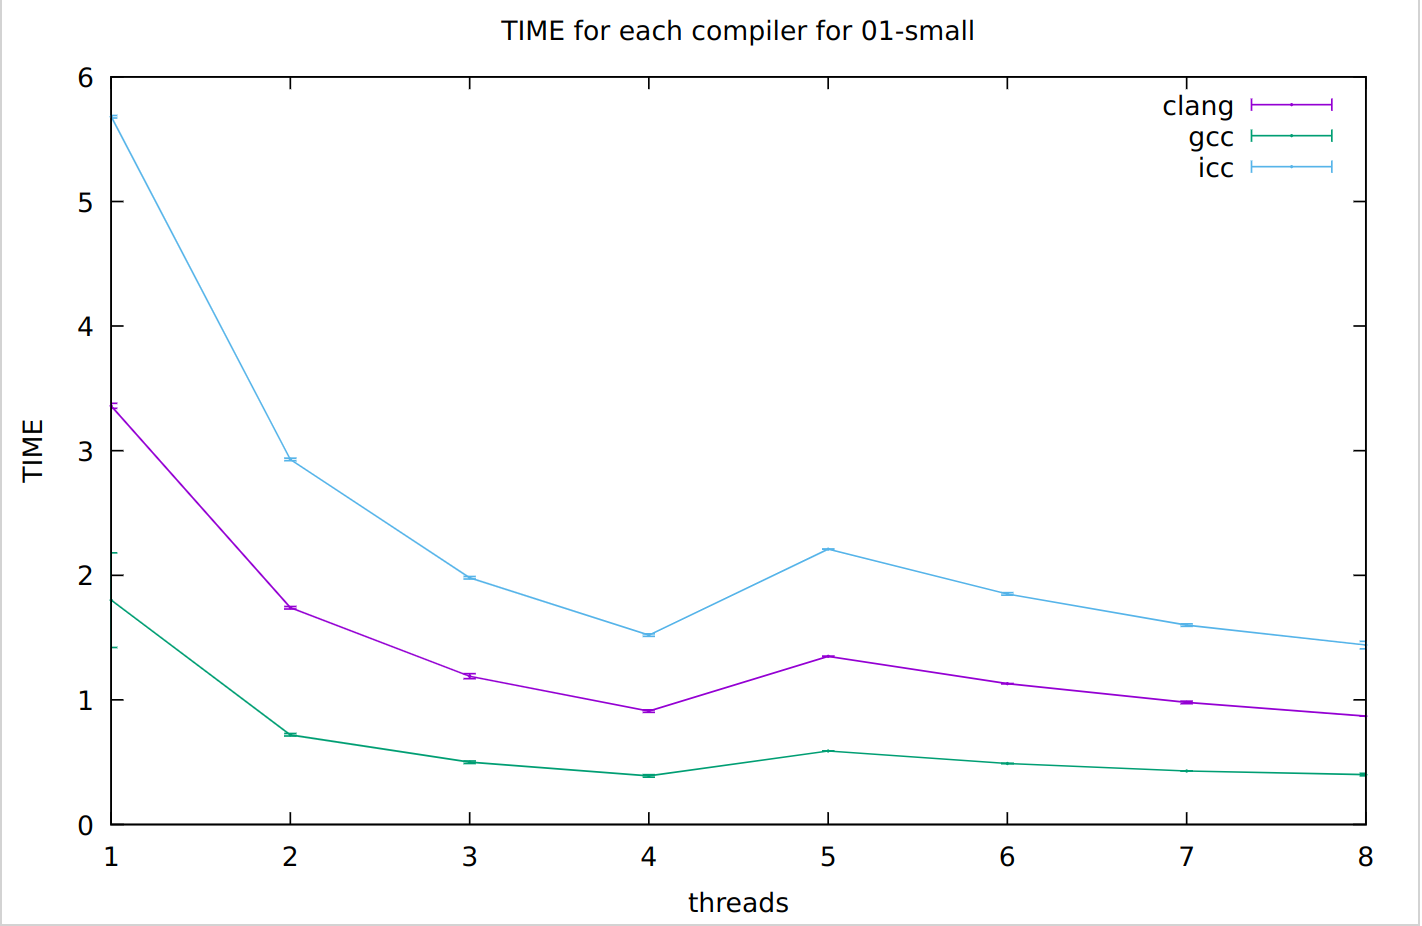
\includegraphics[width=\textwidth]{bucle2-3=01-small}
    \end{subfigure}
    \caption{\underline{Tamaño pequeño}: Tiempos de ejecución vs nº de hilos}
    \label{fig:bucle2-3=01-small}
\end{figure}

%%% TABLA DE TIEMPOS E IMÁGENES %%%
\begin{figure}[H]
    \centering
    \begin{subfigure}{0.4\textwidth}
        \begin{adjustbox}{width=\textwidth} 
        \begin{tabular}{|c|c|c|c|c|}
            \hline
            \rowcolor{azul} \multicolumn{2}{|c|}{}&\multicolumn{3}{c|}{\textbf{Compiler}} \\ \hline
            \rowcolor{azul} \multicolumn{2}{|c|}{}&\texttt{clang}&\texttt{gcc}&\texttt{icc}\\ \hline
            \rowcolor{azul} \textbf{Testing size} & \textbf{Threads}&\multicolumn{3}{c|}{\textbf{Average time (s)}} \\ \hline
            \multirow{8}{2.5cm}{\textbf{02-medium}} & 1 & \(9.68\pm{0.02}\) & \(4.00\pm{0.03}\) & \(16.34\pm{0.03}\) \\ \cline{2-5}
            & 2 & \(4.99\pm{0.03}\) & \(2.06\pm{0.03}\) & \(8.40\pm{0.06}\) \\ \cline{2-5}
            & 3 & \(3.36\pm{0.02}\) & \(1.45\pm{0.08}\) & \(5.65\pm{0.01}\) \\ \cline{2-5}
            & 4 & \(2.59\pm{0.03}\) & \(1.12\pm{0.06}\) & \(4.33\pm{0.02}\) \\ \cline{2-5}
            & 5 & \(3.84\pm{0.00}\) & \(1.66\pm{0.01}\) & \(6.32\pm{0.01}\) \\ \cline{2-5}
            & 6 & \(3.21\pm{0.00}\) & \(1.39\pm{0.00}\) & \(5.28\pm{0.00}\) \\ \cline{2-5}
            & 7 & \(2.76\pm{0.00}\) & \(1.22\pm{0.02}\) & \(4.54\pm{0.01}\) \\ \cline{2-5}
            & 8 & \(2.47\pm{0.01}\) & \(1.09\pm{0.02}\) & \(4.39\pm{0.08}\) \\ \hline
        \end{tabular}
        \end{adjustbox}
    \end{subfigure}
    \hfill
    \begin{subfigure}{0.5\textwidth}
        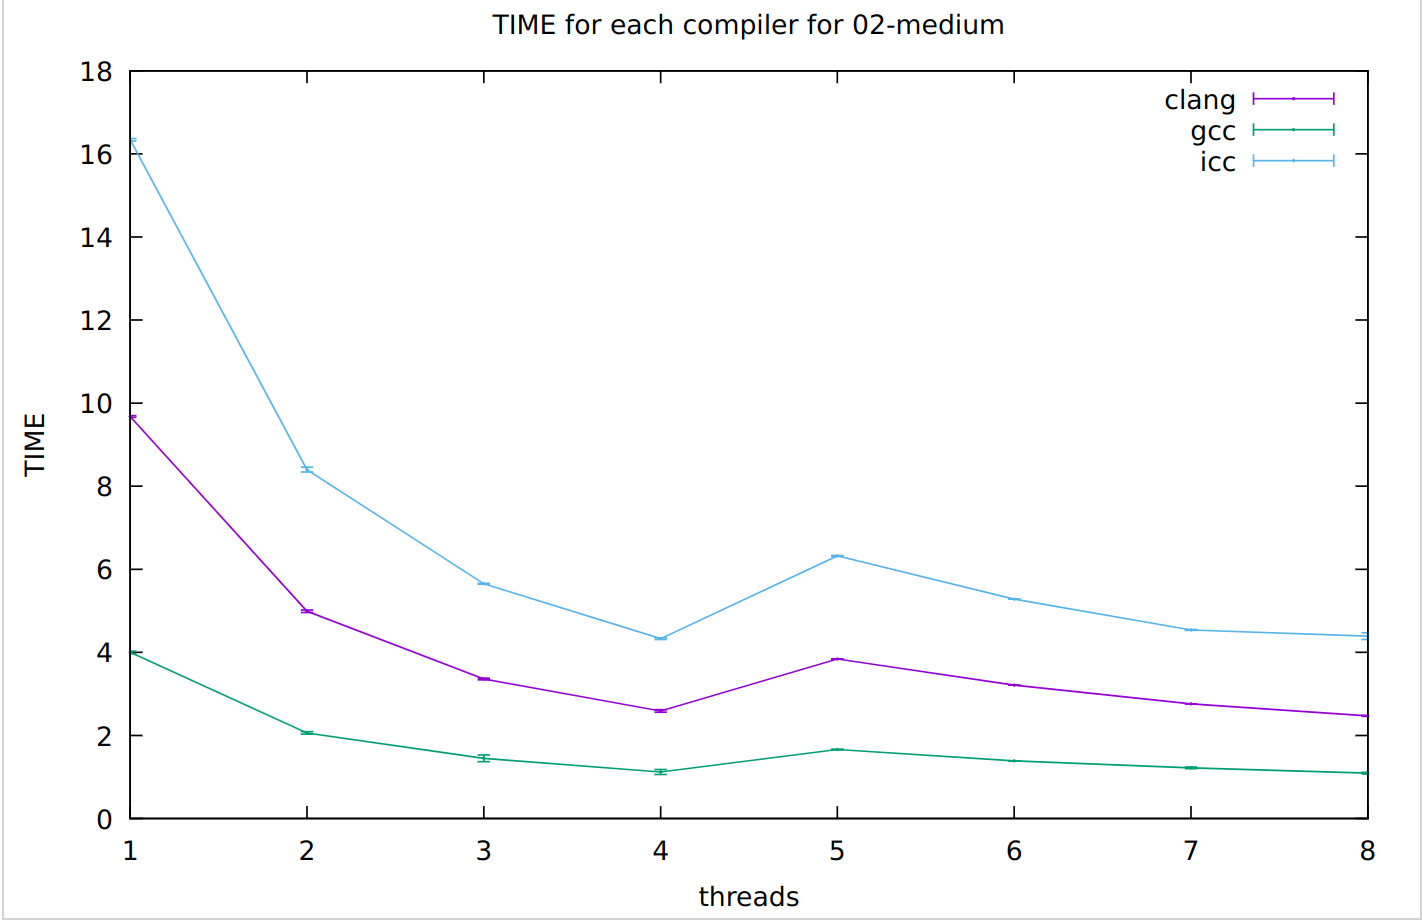
\includegraphics[width=\textwidth]{bucle2-3=02-medium}
    \end{subfigure}
    \caption{\underline{Tamaño mediano}: Tiempos de ejecución vs nº de hilos}
    \label{bucle2-3=02-medium}
\end{figure}

%%% TABLA DE TIEMPOS E IMÁGENES %%%
\begin{figure}[H]
    \centering
    \begin{subfigure}{0.4\textwidth}
        \begin{adjustbox}{width=\textwidth} 
        \begin{tabular}{|c|c|c|c|c|}
            \hline
            \rowcolor{azul} \multicolumn{2}{|c|}{}&\multicolumn{3}{c|}{\textbf{Compiler}} \\ \hline
            \rowcolor{azul} \multicolumn{2}{|c|}{}&\texttt{clang}&\texttt{gcc}&\texttt{icc}\\ \hline
            \rowcolor{azul} \textbf{Testing size} & \textbf{Threads}&\multicolumn{3}{c|}{\textbf{Average time (s)}} \\ \hline
            \multirow{8}{1cm}{\textbf{03-large}} & 1 & \(16.48\pm{0.01}\) & \(6.96\pm{0.12}\) & \(27.84\pm{0.06}\) \\ \cline{2-5}
            & 2 & \(8.54\pm{0.04}\) & \(3.55\pm{0.10}\) & \(14.33\pm{0.07}\) \\ \cline{2-5}
            & 3 & \(5.75\pm{0.00}\) & \(2.39\pm{0.03}\) & \(9.61\pm{0.06}\) \\ \cline{2-5}
            & 4 & \(4.41\pm{0.00}\) & \(1.85\pm{0.06}\) & \(7.35\pm{0.00}\) \\ \cline{2-5}
            & 5 & \(6.60\pm{0.05}\) & \(2.82\pm{0.01}\) & \(10.79\pm{0.02}\) \\ \cline{2-5}
            & 6 & \(5.48\pm{0.01}\) & \(2.36\pm{0.01}\) & \(8.99\pm{0.01}\) \\ \cline{2-5}
            & 7 & \(4.69\pm{0.02}\) & \(2.03\pm{0.01}\) & \(7.72\pm{0.00}\) \\ \cline{2-5}
            & 8 & \(4.16\pm{0.00}\) & \(1.82\pm{0.03}\) & \(6.90\pm{0.04}\) \\ \hline
        \end{tabular}
        \end{adjustbox}
    \end{subfigure}
    \hfill
    \begin{subfigure}{0.5\textwidth}
        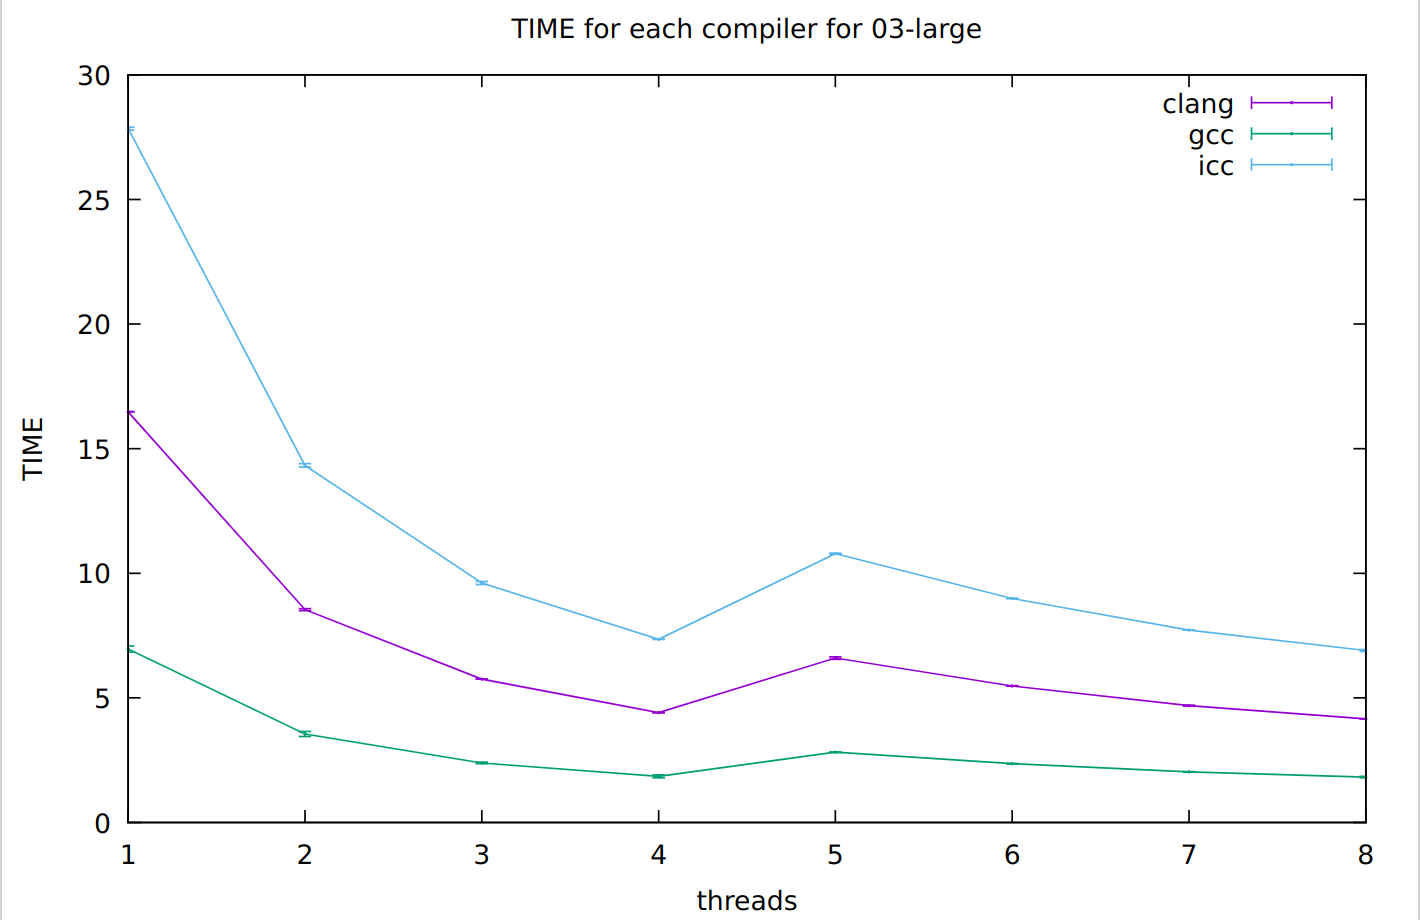
\includegraphics[width=\textwidth]{bucle2-3=03-large}
    \end{subfigure}
    \caption{\underline{Tamaño largo}: Tiempos de ejecución vs nº de hilos}
    \label{bucle2-3=03-large}
\end{figure}

